\section{Parallel Learning and Fresh Held-Out Results}
Actual execution reached the full $500,000$-transition budget with eight environments and one shared policy. Of these, $497,600$ transitions entered completed PPO optimization buffers. The framework received $499,992$ transitions; the remaining eight executed transitions belonged to the failed I/O return boundary and were charged to the cap. The initial $2,400$ executed transitions were discarded from optimization, not counted as a second independent training run. Training used $2,500,000$ native physics steps; the complete campaign, including validation and evaluation, used $2,874,510$ native steps.

The resumed lineage produced $124$ rollout buffers and $612$ recorded epoch counters, with $38271$ gradient/optimizer minibatches. Independent GAE reconstruction had maximum discrepancy $8.94\times10^{-8}$. Behavior-density replay at five saved rollout boundaries had maximum log-probability discrepancy $1.43\times10^{-6}$. Actor and critic parameter changes were nonzero and finite. The $400$ logged post-recovery training episodes reached their configured time limits. All four curriculum levels were used; no no-curriculum ablation establishes its causal contribution. Raw learning curves distinguish changing episode horizons from improved behavior.

The charged training wall time was $892.242$ s, including conservative prior-attempt charge; measured resumed learn/update calls accounted for $818.868$ s. The resulting collection/update throughput was approximately $607.67$ transitions/s for those calls, rather than the earlier environment-only pilot value. Evaluation and rendering are reported separately.

Checkpoint selection used only the fixed development cases, prioritizing full-task passes, passed windows, RMSE, then energy. All reached checkpoints retained fifteen windows on both development cases. The $500,000$ checkpoint was selected by the registered RMSE tie-break among those outcomes and was frozen before final testing. It completed $30$ s without reported physical violation on all three fresh held-out contexts, but passed only fifteen windows in each: full-task success was $0/3$. The exact binomial $95\%$ interval $[0,0.7076]$ is conditional on its trial assumptions and does not represent uncertainty across independently trained policies.

Relative to paired frozen V4, nominal held-out RMSE changes were $-47.777$, $-32.168$, and $-44.051$ micrometres. Corresponding mean modal-energy changes were approximately $-0.1078\%$, $+0.0966\%$, and $-0.2633\%$. These effects were not subjected to a new paired timestep refinement. Two cases were nominally better in both metrics, while one exchanged better tracking for higher energy. Neither the unresolved window nor these small effects supports a claim of consistent superiority. All held-out pairs and unfavorable development checkpoints remain in the evidence package.

\begin{figure*}[t]\centering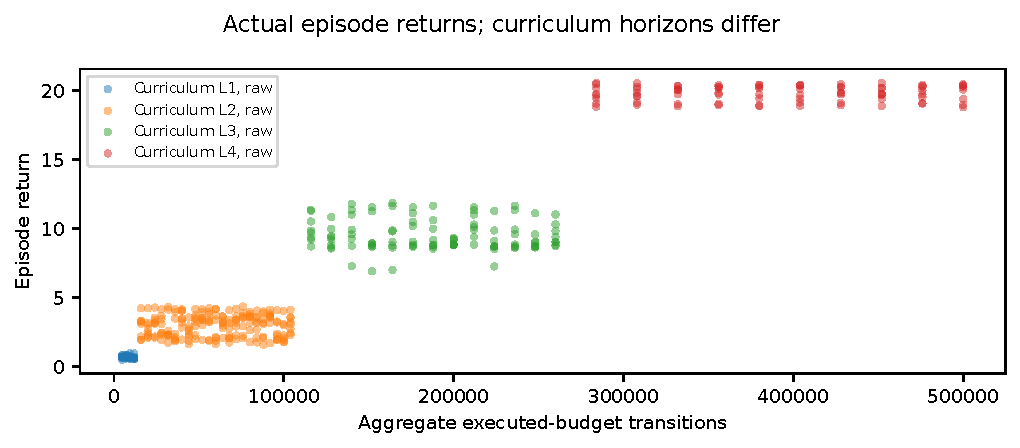
\includegraphics[width=.48\textwidth]{figures/e2e_04_reward.pdf}\hfill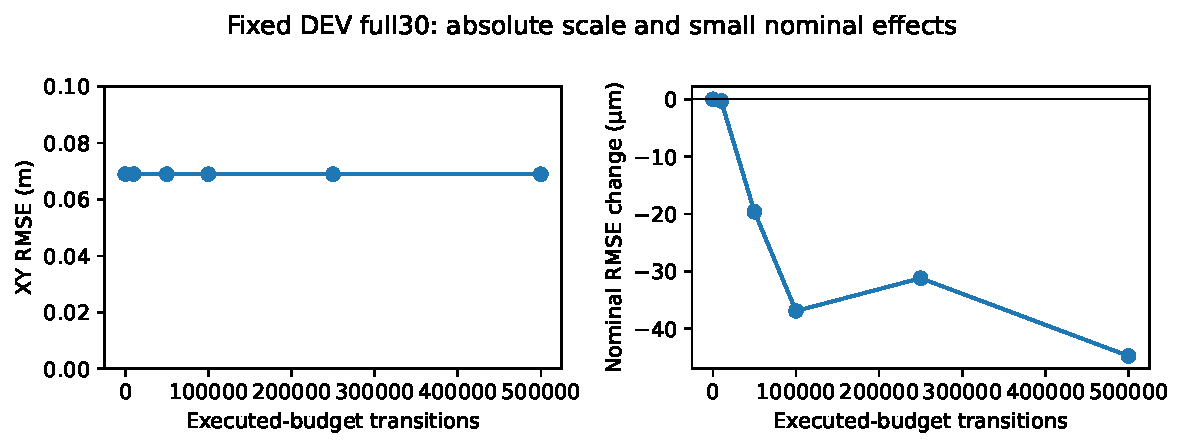
\includegraphics[width=.48\textwidth]{figures/e2e_05_tracking.pdf}\caption{Actual training episode returns and fixed development full-horizon tracking. Curriculum horizons are labeled; return growth is not treated as task success.}\end{figure*}
\begin{figure*}[t]\centering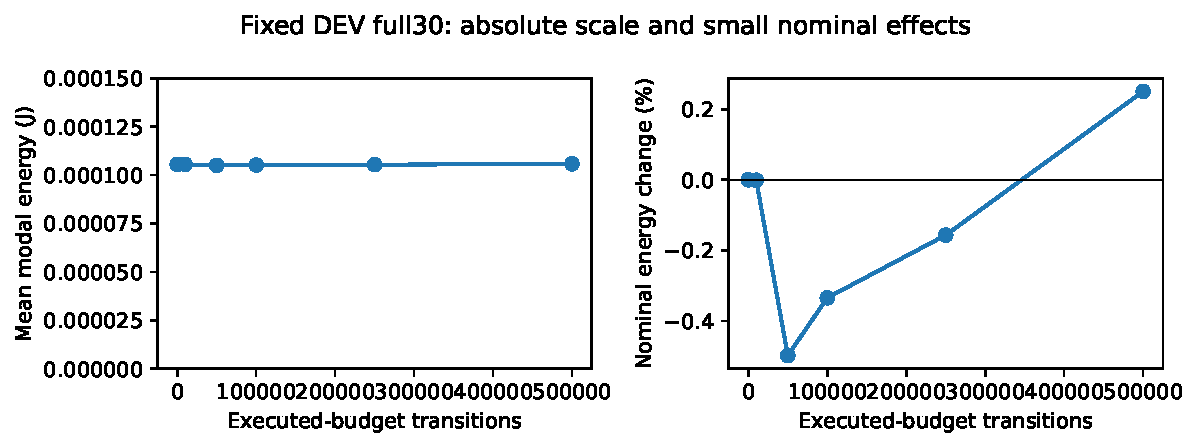
\includegraphics[width=.48\textwidth]{figures/e2e_06_sloshing.pdf}\hfill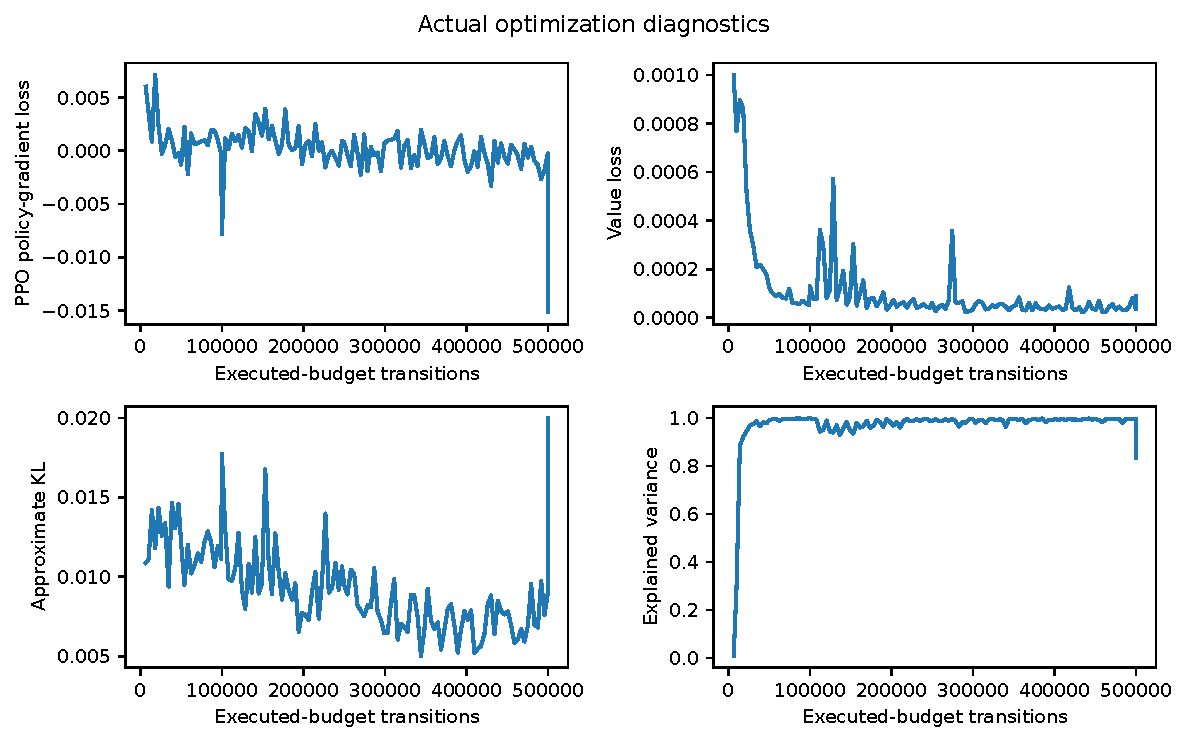
\includegraphics[width=.48\textwidth]{figures/e2e_13_PPO_diagnostics.pdf}\caption{Development modal energy and real optimizer diagnostics. The held-out set was not used to choose checkpoints.}\end{figure*}
\begin{figure*}[t]\centering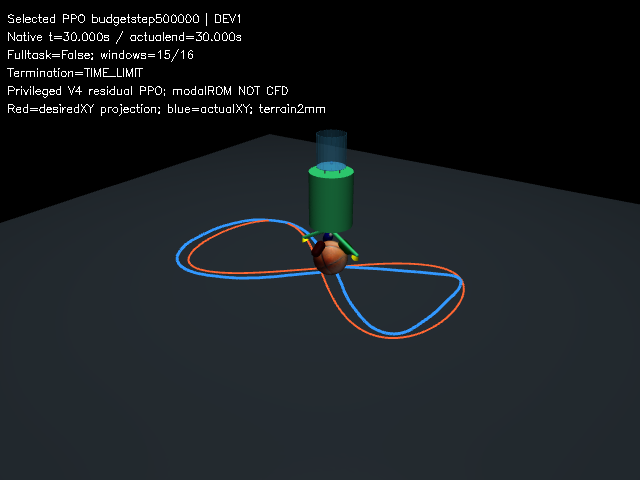
\includegraphics[width=.48\textwidth]{figures/e2e_native.png}\hfill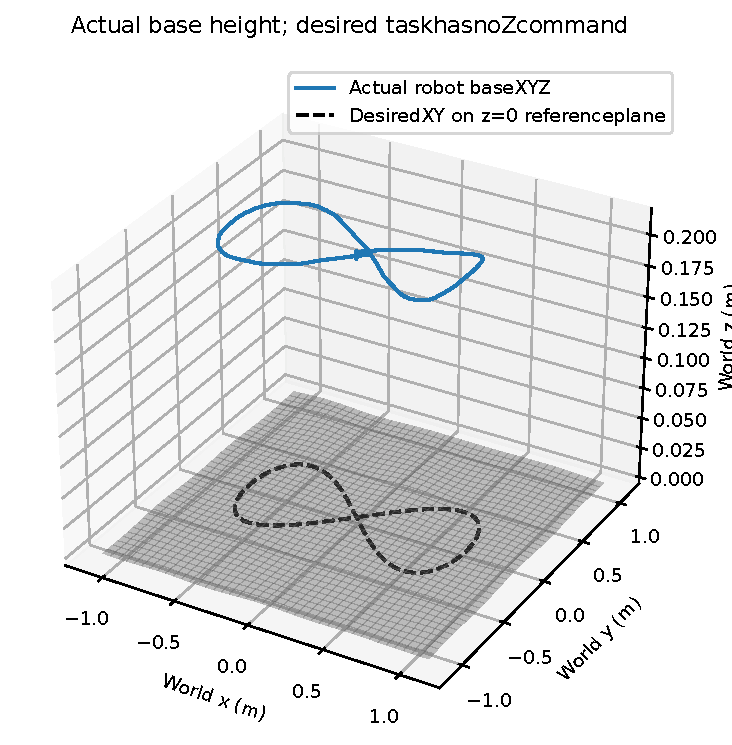
\includegraphics[width=.48\textwidth]{figures/e2e_11_3D.pdf}\caption{Actual native MuJoCo replay and recorded base height on the unexaggerated terrain. The liquid visualization is a modal surrogate, not a resolved fluid surface.}\end{figure*}
